\documentclass[11pt,a4paper]{article}

% French
\usepackage[utf8x]{inputenc}
\usepackage[frenchb]{babel}
\usepackage[T1]{fontenc}
\usepackage{lmodern}
\usepackage{ifthen}

% Color
% cfr http://en.wikibooks.org/wiki/LaTeX/Colors
\usepackage{color}
\usepackage[usenames,dvipsnames,svgnames,table]{xcolor}
\definecolor{dkgreen}{rgb}{0.25,0.7,0.35}
\definecolor{dkred}{rgb}{0.7,0,0}

% Floats and referencing
\newcommand{\sectionref}[1]{section~\ref{sec:#1}}
\newcommand{\annexeref}[1]{annexe~\ref{ann:#1}}
\newcommand{\figuref}[1]{figure~\ref{fig:#1}}
\newcommand{\tabref}[1]{table~\ref{tab:#1}}
\usepackage{xparse}
\NewDocumentEnvironment{myfig}{mm}
{\begin{figure}[!ht]\centering}
{\caption{#2}\label{fig:#1}\end{figure}}

% Listing
\usepackage{listings}
\lstset{
  numbers=left,
  numberstyle=\tiny\color{gray},
  basicstyle=\rm\small\ttfamily,
  keywordstyle=\bfseries\color{dkred},
  frame=single,
  commentstyle=\color{gray}=small,
  stringstyle=\color{dkgreen},
  %backgroundcolor=\color{gray!10},
  %tabsize=2,
  rulecolor=\color{black!30},
  %title=\lstname,
  breaklines=true,
  framextopmargin=2pt,
  framexbottommargin=2pt,
  extendedchars=true,
  inputencoding=utf8x
}

\newcommand{\matlab}{\textsc{Matlab}}
\newcommand{\octave}{\textsc{GNU/Octave}}
\newcommand{\qtoctave}{\textsc{QtOctave}}
\newcommand{\oz}{\textsc{Oz}}
\newcommand{\java}{\textsc{Java}}
\newcommand{\clang}{\textsc{C}}
\newcommand{\keyword}{mot clef}

% Math symbols
\usepackage{amsmath}
\usepackage{amssymb}
\usepackage{amsthm}
\DeclareMathOperator*{\argmin}{arg\,min}
\DeclareMathOperator*{\argmax}{arg\,max}

% Sets
\newcommand{\Z}{\mathbb{Z}}
\newcommand{\R}{\mathbb{R}}
\newcommand{\Rn}{\R^n}
\newcommand{\Rnn}{\R^{n \times n}}
\newcommand{\C}{\mathbb{C}}
\newcommand{\K}{\mathbb{K}}
\newcommand{\Kn}{\K^n}
\newcommand{\Knn}{\K^{n \times n}}

% Chemistry
\newcommand{\std}{\ensuremath{^{\circ}}}
\newcommand\ph{\ensuremath{\mathrm{pH}}}

% Theorem and definitions
\theoremstyle{definition}
\newtheorem{mydef}{Définition}
\newtheorem{mynota}[mydef]{Notation}
\newtheorem{myprop}[mydef]{Propriétés}
\newtheorem{myrem}[mydef]{Remarque}
\newtheorem{myform}[mydef]{Formules}
\newtheorem{mycorr}[mydef]{Corrolaire}
\newtheorem{mytheo}[mydef]{Théorème}
\newtheorem{mylem}[mydef]{Lemme}
\newtheorem{myexem}[mydef]{Exemple}
\newtheorem{myineg}[mydef]{Inégalité}

% Unit vectors
\usepackage{esint}
\usepackage{esvect}
\newcommand{\kmath}{k}
\newcommand{\xunit}{\hat{\imath}}
\newcommand{\yunit}{\hat{\jmath}}
\newcommand{\zunit}{\hat{\kmath}}

% rot & div & grad & lap
\DeclareMathOperator{\newdiv}{div}
\newcommand{\divn}[1]{\nabla \cdot #1}
\newcommand{\rotn}[1]{\nabla \times #1}
\newcommand{\grad}[1]{\nabla #1}
\newcommand{\gradn}[1]{\nabla #1}
\newcommand{\lap}[1]{\nabla^2 #1}


% Elec
\newcommand{\B}{\vec B}
\newcommand{\E}{\vec E}
\newcommand{\EMF}{\mathcal{E}}
\newcommand{\perm}{\varepsilon} % permittivity

\newcommand{\bigoh}{\mathcal{O}}
\newcommand\eqdef{\triangleq}

\DeclareMathOperator{\newdiff}{d} % use \dif instead
\newcommand{\dif}{\newdiff\!}
\newcommand{\fpart}[2]{\frac{\partial #1}{\partial #2}}
\newcommand{\ffpart}[2]{\frac{\partial^2 #1}{\partial #2^2}}
\newcommand{\fdpart}[3]{\frac{\partial^2 #1}{\partial #2\partial #3}}
\newcommand{\fdif}[2]{\frac{\dif #1}{\dif #2}}
\newcommand{\ffdif}[2]{\frac{\dif^2 #1}{\dif #2^2}}
\newcommand{\constant}{\ensuremath{\mathrm{cst}}}

% Numbers and units
\usepackage[squaren, Gray]{SIunits}
\usepackage{sistyle}
\usepackage[autolanguage]{numprint}
%\usepackage{numprint}
\newcommand\si[2]{\numprint[#2]{#1}}
\newcommand\np[1]{\numprint{#1}}

\newcommand\strong[1]{\textbf{#1}}
\newcommand{\annexe}{\part{Annexes}\appendix}

% Bibliography
\newcommand{\biblio}{\bibliographystyle{plain}\bibliography{biblio}}

\usepackage{fullpage}
% le `[e ]' rend le premier argument (#1) optionnel
% avec comme valeur par défaut `e `
\newcommand{\hypertitle}[7][e ]{
\usepackage{hyperref}
{\renewcommand{\and}{\unskip, }
\hypersetup{pdfauthor={#6},
            pdftitle={Synth\`ese d#1#2 Q#3 - L#4#5},
            pdfsubject={#2}}
}

\title{Synth\`ese d#1#2 Q#3 - L#4#5}
\author{#6}

\begin{document}

\ifthenelse{\isundefined{\skiptitlepage}}{
\begin{titlepage}
\maketitle

 \paragraph{Informations importantes}
   Ce document est grandement inspiré de l'excellent cours
   donné par #7 à l'EPL (École Polytechnique de Louvain),
   faculté de l'UCL (Université Catholique de Louvain).
   Il est écrit par les auteurs susnommés avec l'aide de tous
   les autres étudiants, la vôtre est donc la bienvenue.
   Il y a toujours moyen de l'améliorer, surtout si le cours
   change car la synthèse doit alors être modifiée en conséquence.
   On peut retrouver le code source à l'adresse suivante
   \begin{center}
     \url{https://github.com/Gp2mv3/Syntheses}.
   \end{center}
   On y trouve aussi le contenu du \texttt{README} qui contient de plus
   amples informations, vous êtes invité à le lire.

   Il y est indiqué que les questions, signalements d'erreurs,
   suggestions d'améliorations ou quelque discussion que ce soit
   relative au projet
   sont à spécifier de préférence à l'adresse suivante
   \begin{center}
     \url{https://github.com/Gp2mv3/Syntheses/issues}.
   \end{center}
   Ça permet à tout le monde de les voir, les commenter et agir
   en conséquence.
   Vous êtes d'ailleurs invité à participer aux discussions.

   Vous trouverez aussi des informations dans le wiki
   \begin{center}
     \url{https://github.com/Gp2mv3/Syntheses/wiki}.
   \end{center}
   comme le statut des synthèses pour chaque cours
   \begin{center}
     \url{https://github.com/Gp2mv3/Syntheses/wiki/Status}.
   \end{center}
   vous pouvez d'ailleurs remarquer qu'il en manque encore beaucoup,
   votre aide est la bienvenue.

   Pour contribuer au bug tracker et au wiki, il vous suffira de
   créer un compte sur Github.
   Pour interagir avec le code des synthèses,
   il vous faudra installer \LaTeX.
   Pour interagir directement avec le code sur Github,
   vous devez utiliser \texttt{git}.
   Si cela pose problème,
   nous sommes évidemment ouverts à des contributeurs envoyant leurs
   changements par mail ou n'importe quel autre moyen.
\end{titlepage}
}{}

\ifthenelse{\isundefined{\skiptableofcontents}}{
\tableofcontents
}{}
}


\usepackage{multirow}
\usepackage{multicol}
\usepackage{graphicx}

% Footnote in tabular
\usepackage{footnote}
\makesavenoteenv{tabular}
\makesavenoteenv{table}

\hypertitle{en}{Computer Networks : Information transfer}{5}{INGI}{1341}
{Nicolas Houtain\and Benoît Legat}
{Olivier Bonaventure}

\paragraph{French}
There is some part in french because this is a merge between 2 summaries.
It needs to be translated.

\section{Terminology}

\begin{description}
    \item[PDU] : \textit{Protocole data unit}. Unité de mesure des informations échangées
        dans un réseau informatique.


    \item[DNS] : \textit{Domain Name System}. Service permettant de traduire un nom de domaine en informations de plusieurs types qui y sont associées, notamment une IP.
    \item[DIFS] : \textit{DCF Interframe Space}. Si une station détecte qu'il n'y a pas eu de transmission WiFi pendant DIFS microsecondes et que l'échange de la dernière trame a réussi, elle a le droit de transmettre. Cette valeur au sein de la gestion des collisions : DIFS = SIFS + (2 * Slot time)
    \item[EIFS] : \textit{Extended Interframe Space}. Similaire au DIFS mais activé uniquement si la dernière frame a échoué. EIFS = Temps de transmission d'un acquittement + SIFS + DIFS.
    \item[HTTP] : \textit{HyperText Transfer Protocol}
    \item[RIFS] : \textit{Reduced Interframe Space}.
    \item[SDU] : \textit{Service Data Unit}
    \item[SIFS] : \textit{Short Inter Frame Spacing}. Temps pour une interface sans-fil entre la gestion d'une trame reçue et l'envoi de l'acquittement correspondant (temps pour passer de download à upload pour un routeur).  -> CSMA/CA
    \item[TLV] : \textit{Type Length Value} est un format d'encodage tel que le premier byte est le type, le second la taille totale et puis la valeur.
\end{description}

\section{Layers}

The different layers are represented by the \tabref{layers}.
A router only has the 3 layers: Network, Datalink and Physical.
\begin{table}[!ht]
  \centering
  \begin{tabular}{|c|c|c|p{4cm}|c|c|}
    \hline
    \multicolumn{3}{|c|}{Layers} & Protocols & PDU\footnote{Protocol Data Unit} & Id\footnote{I know it is a bit an overgeneralization.}\\
    \cline{1-3}
    CNP3 & TCP/IP & OSI & & & \\
    \hline
    \multirow{3}{*}{Application} & \multirow{3}{*}{Application}             & Application  & BGP, DHCP, DNS, FTP, HTTP, NFS, NTP, RIP, SMTP, SNMP, Telnet & ADU & \\
    \cline{3-6}
                                 &                                          & Presentation & MIME, XDR, SSL & & \\
    \cline{3-6}
                                 &                                          & Session      & RTP, TLS & SDU & \\
    \hline
    Transport                    & Transport                                & Transport    & UDP, MPTCP, TCP, SCTP & segment & Port\\
    \hline
    Network                      & Internet                                 & Network      & ICMP, IPsec, IPv4, IPv6, IPX, MPLS\footnote{MultiProtocol Label Switching operates at a layer that is generally considered to lie between traditional definitions of layer 2 (data link layer) and layer 3 (network layer), and thus is often referred to as a ``layer 2.5'' protocol} & packet & IP\\
    \hline
    Datalink                     & \multirow{2}{*}{Link}                    & Datalink     & IEEE 802.3 (Ethernet), IEEE 802.4, IEEE 802.5, ATM, ARP, Frame Relay, HDLC, IS-IS, LAPB, LLC, MAC, OSPF, PPP, SLIP & frame & MAC\\
    \cline{1-1}
    \cline{3-6}
    Physical                     &                                          & Physical     & DSL, IEEE 802.3 (Ethernet), IEEE 802.11 (WiFi), ISDN, Modems & bit & \\
    \hline
  \end{tabular}
  \caption{This table contains all the protocols of \cite{bonaventure2011computer}. See \cite{wiki:osimodel} for more protocols.}
  \label{tab:layers}
\end{table}

\begin{myexem}
  An HTTPS request will use the following protocols in each layer of the OSI model:
  \begin{description}
    \item[Application] HTTP,
    \item[Presentation] SSL,
    \item[Session] TLS,
    \item[Transport] TCP,
    \item[Network] IPv6,
    \item[Datalink] IEEE 802.3 (Ethernet),
    \item[Physical] IEEE 802.3 or IEEE 802.11 (Wireless Local Area Network).
  \end{description}
\end{myexem}

\subsection{Physical Layer}
The Physical Layer service is provided by
\begin{itemize}
  \item \textbf{Electrical cable} twisted pairs or coaxial cables;
  \item \textbf{Optical fiber} multimode or monomode;
  \item \textbf{Wireless} laser for point-to-point and radio-based for spread signal (e.g. WIFI).
\end{itemize}
Its PDU is the bit and the following terms are used
\begin{itemize}
    \item \textbf{Bit rate} : Expressed in bits/sec
    \item \textbf{Bandwith} : Range of frequency usable
\end{itemize}

\subsubsection{Characteristic}

It is \textit{not perfect} (unreliable),
and for us it is like a black box with these characteristics :
\begin{itemize}
    \item \textcolor{red}{change} the value of a bit (\textit{car interference electromagnétique});
    \item deliver \textcolor{red}{more or fewer} bits than requested (\textit{car frequence horloge imprécise})
\end{itemize}

\paragraph{Manchester encoding}
It's an encoding that consist in dividing time in fixed length period. To send a 1, the voltage must be high in the first half of a period and the become low (opposite for zero). It use the symbol InvH (high voltage during last period) and InvB as special marker.

\subsection{Datalink Layer}
The PDU of Datalink Layer service is a \textbf{frame} (\textit{sequence of bit with a particular syntax or structure}) because we want to share data block.
A frame is separated in 3 parts :
\begin{itemize}
    \item \textbf{Header} It contains a flag to tell whether it is an \textcolor{red}{ACK or DATA}, a \textcolor{red}{sequence number} and sometimes the length of the payload.
  \item \textbf{Payload} It contains the information that needs to be transmitted.
  \item \textbf{Error Detection Code} It allows the receiver to detect transmission errors.
    It is either
    \begin{itemize}
        \item a \textsc{hamming code} which is simply a parity bit, it can only detect odd number of errors;
        \item a \textsc{checksum such} as the Internet checksum chosen by the TCP/IP community and the
        Fletcher checksum chosen by the OSI community;
    \item or a \textsc{Cyclic Redundancy Check} (CRC).
        It was slow to implement in software before 1995 and the publication of \cite{feldmeier1995fast}.
        It is now preferred since it has better error detection \cite{stone1998performance}.
        An $n$ bit CRC can detect errors if there are at most $n$
        bits in error or if there is an odd number of bits in error.
    \item an \textsc{hash function} like MD5 or SHA: however, these are built to be collision resistant against
        an active adversary, not random modifications.
        They are also a lot slower than CRC or checksums so they are only used in cryptography.
    \end{itemize}
  \item \textbf{Error Correction Code} It allow the receiver to correct transmission errors.
    No widely used datalink protocol use this.
\end{itemize}

\subsubsection{Framing}

The separation of frames are done using \emph{bit stuffing}
or \emph{character stuffing}.

\begin{description}
    \item[Bit stuffing] : \textbf{01111110} is a frame \textcolor{red}{boundary marker}, so he can't
    be used when we transmit frames.
    \textit{Adds a 0 after 5 consecutive 1 to ensure that this marker is not in the frame}
    \begin{enumerate}
      \item Easy to implement in hardware.
      \item Increase number of bit transmited
    \end{enumerate}
\item[Character stuffing] : In software it's easier to work with character. 
    (No imprimable character use as marker)
    Begin of frame : \textsc{DLE STX}, end of frame : \textsc{DLE ETX}.
\end{description}

\paragraph{Note} : Bit stuffing is implemented in hardware and character stuffing is usually
implemented in software.

\subsubsection{Recovering from failures}
We can have errors due to different events:
\begin{enumerate}
  \item The frame has been \textbf{lost} or has been \textbf{corrupted}
    by a transmission error
  \item When we are to slow to treat incoming frames (\textbf{overflow} of the buffer)
\end{enumerate}

\paragraph{ }
Thanks to the ACK flag in the header,
we have 2 types of frames: \textbf{data frame} and \textbf{acknowledgment frame}.
Using to the  \textbf{Error Detection Code}, we can try  to recover from failures
of the physical layers and provide a reliable service.

\paragraph{Note: }
Since the \textbf{Physical Layer does not reorder} the bits,
the frames will not be reordered either.
Providing a reliable service it therefore easier than for the Transport Layer that has to cope with the reordering of packets in the Network Layer (it has to discard packets to old packets and have maximal throughput because of that).

\paragraph{Pipelling:  }  This technique  allows  a  sender to  transmit
several  consecutive frames  without being  forced to  wait for  and ack
after each frame.

\subsubsection{Reliable datalink layer}
There are 3 ways of achieving a reliable Datalink Layer.
\begin{enumerate}
  \item \textbf{ABP} :
    The Alternating Bit Protocol is
    a particular case of go-back-n for $n = 2$.
  \item \textbf{Go-back-n} :
    is simple, the receiver discards all out of sequence frames
    and the ACK always contains the last in sequence frame received.

    The sender has simply one timer and when it expires, it retransmits \emph{all}
    its unacked frames.

    \begin{center}
    \textit{Good performance if few frame are lost but else the performance is quickly
    drop because of out-sequence frame not accepted and retransmittion of all
unacked frames when it has detected a loss.}
\end{center}

  \item \textbf{Selective Repeat}
      The difference with the go-back-n is that the receiver \textbf{stored out of sequence} frames received, even if cumulative acknowledgement is still used. (\textit{ACK
      contains yet the last in sequence frame received even a out of sequence
  frame is store in buffer})

    The sender has  now a timer  for each frame  of the
    sending window.

    \begin{itemize}
        \item[$\to$] The ACK sometimes also contains the list of out of sequence frame received (\emph{selective acknowledgement}) to avoid useless retransmission.
    \end{itemize}
\end{enumerate}

\paragraph{Buffer size}
If the sequence number has $n$ bits, we use $2^n$ \textbf{different sequence} numbers.
A \textit{Sliding window} is use to manage the buffer of sequence numbers.

Because the Physical Layer will not reorder the frames,
the maximum window size for the go-back-n is $\bf 2^n-1$ and is $\bf 2^{n-1}$ for the Selective Repeat.

\paragraph{  }  Not  all  Datalink Services  provide  a  \emph{reliable}
service. As  a rule  of thumb, datalink  services above  very unreliable
wireless physical services  (e.g. WIFI) does provide  a reliable service
and datalink services above almost reliable wired physical sercies (e.g.
cable or fiber)  do dot include additional  retransmission mechanism and
are also \emph{almost reliable}.

\paragraph{Piggybacking}
When DATA is sent in both directions, an ACK frame and a DATA frame sent by one side are sometimes merged in one because an ACK frame does not need a lot of bit to do its job.
(\textit{Used to reduce the overhead caused by acknowledgements})


\subsubsection{Medium Access Control (MAC)}
The first of the 3 resources that need to be shared inside a network is the link bandwidth (the 2 others are routers processing time and routers buffers).

\textsc{Collisions} happens when two hosts try to send a frame simultaneously.
It is the principal source of errors in Local Area Network.

There are 2 types of MAC, deterministic ones and stochastic ones.
\begin{itemize}
  \item deterministic or pessimistic MACs: They ensure that there will be \emph{no} collision.
    They are more appropriate in network where the load is constant (e.g. telephone, radio).
  \item stochastics or optimistic MACS: They try to minimize the number of collisions.
    They are more appropriate in network where the load has an on-off behaviour (e.g. internet).
\end{itemize}

The deterministic MACs are the following (the 3 first are \emph{static} allocation methods)
\begin{description}
  \item[Frequency Division Multiplexing]
    If wireless medium, we can give a different frequency for devices.
  \item[Wavelength Division Multiplexing]
    In optical medium, we can give a different wavelength for devices.
  \item[Time Division Multiplexing]
    In any medium, we can just divide the time in separate slots and assign the slots to devices
    statically or dynamically.
  \item[IEEE 802.4 (Token Bus Network)]
    Transmit a token in a network of bus topology.
    To transmit data, wait for the token and then transmit the data instead of the token.
    Once the data transmitted, put the token back in the network.
  \item[IEEE 802.5 (Token Ring Network)]
    Same than 802.4 but with a ring topology.
\end{description}

\paragraph{[slotted] ALOHA}
The first approach is ALOHA.
The idea is simple.
When no ack is received, we wait a random time instead of a fixed time to avoid synchronisation with other hosts.
A simple improvement is \emph{slotted} ALOHA which divides the times into slots of the same size than the time require to transmit one frame.
Transmisssion are only allowed to start at the beginning of a time slot.
This avoids collison on part of a frame since that require the frame to be completely retransmitted anyway.

\paragraph{[non-]persistent CSMA}
An improvement to ALOHA is \emph{persistent} CSMA which sense the network before sending a frame but does not wait random time.
To avoid synchronisation on with CSMA, \emph{non-persistent} CSMA waits a random time before sensing the network,
it is is not free, it will wait a random time before sensing it again.

More improvements can be made but depends on the technology
\paragraph{CSMA/CD for IEEE 802.3 (Ethernet)}
On ethernet, a host is able to detect a collision while it is listening.
If $\tau$ is the diameter of the network (the largest time between 2 host),
we know that if a frame of length $2\tau$ has a collision, the sending host will sense it (as any other hosts by the way).
We therefore enforce $2\tau$ as the minimum frame size.

Since Ethernet has not many transmission errors, CSMA/CD does not uses acknowledgment to avoid the collisions they would cause.

The time waited by the hosts when a collision is detected is random to avoid synchronisation,
is a multiple of $2\tau$ for the same reason as slotted ALOHA and is selected in a range multiplied by 2 after each collision,
this is called a \emph{binary exponential back-off}.

\paragraph{CSMA/CA for IEEE 802.11 (WiFi)}

\begin{description}
  \item[sifs] this is required to switch between upload and download in a router.
  \item[difs]
  \item[eifs]
\end{description}

% Network:
% Datagram: connectionless-> most
% Virtual circuit: connection-> few
%
% Transport
% most on top on datagram so
% UDP: datagraph: connectionless
% TCP: connection oriented
% UDP
%
% Resource Sharing
% Resources that need to be shared:
% * Links Bandwidth
% * Buffers on the network nodes
% * Packet processing capacity of nodes



\subsection{Building a network}
Network layer is used to send packet between two host that cannot directly relied
by a cable. Host and router \textbf{sending packet}.

There are two possible organisation for the network layer.

\begin{itemize}
    \item \textbf{Data plane :} Protocol and algorithm use to forward data
    \item \textbf{Control plane :} Protocol and algorithm use to make forwarding table
\end{itemize}

\subsubsection{The datagram organisation}

\textit{Inspired by the postal service}, each host is identified by a \textbf{network layer address}.

For each \textsc{packet}, sender must define his address, receiver address and data.

\paragraph{Forwarding}
In datagram organisation, router use \textbf{hop-by-hop} forwarding. (\textit{Each router
forward the packet with his forwarding table})

In a network, \textbf{black-hole} (\textit{when router discard packet because not entry
in his forwarding table for this destination}) and \textbf{cycle} ({packet
consume bandwith}) must be avoiding!


\paragraph{Computing forwarding tables}

\begin{description}
    \item[Port-address table] : Only if we have a \textbf{tree-shapped network} (\textit{drawback}), il suffit d'inspecter les packets reçu pour créer sa table de forwarding sans risquer d'avoir de loop.
        \begin{enumerate}
            \item If the destination address is in the forwarding table, the packet is
                forward on the right interface
            \item Else the packet is send on all interface except the interface
                from wich the packet was receive. It's call \textbf{broadcasting}
                (\textit{drawback})
        \end{enumerate}

        $\to$ The problem with a tree-shapped network is that if a link fails, the network is \textit{split} in two network since there is no redundancy.

        \begin{center}
            \textit{If the network is not a tree, we can also use port-address table but we need to use a distributed algorithm to ensure
            that we have a tree (e.g. Spanning Tree Protocol for Ethernet (Datalink Layer)).}
        \end{center}

    \item[Source routing] : There is no destination address but only the path to reach
        the destination host. Two type of packet :
        \begin{enumerate}
            \item Data packet : to exchange data
            \item Control packet : to discover the path between endhosts. 
                When a router receive a control packet he forwad this one via
                all interface.

                Avoid possible loop because control packet contains a list of \textbf{intermediate nodes}.
        \end{enumerate}
        Complexity is placed on the endhost and network node is simpliest.

\end{description}

\paragraph{Flat or hierachical adresse}
Flat is like number telephone (small match to forwad packet) and hierachical is like a postal adress (smaller forwarding table but adress change when attached to other node\ldots issues with mobile host).

\paragraph{Dealing with heterogeneous datalink}

\begin{enumerate}
    \item \textbf{Retransmitting} : Discard packet and send a control packet to the source to indicate that it cannot forward pacjets longer than 500byte. Source retransmitting the informaiton in smaller packer.
        \begin{center}
            \textit{Router can be really simple and no additionnal operation to perform,
            but may be inefficient because of retransmitting}
        \end{center}
    \item \textbf{Fragmenting} : Router can fragment packet, to way to achieve this :
        \begin{enumerate}
            \item The next router reassembles the fragment
                \begin{center}
                    \textit{Take so much CPU time and memory to fragment 
                    and after reassemble}
                \end{center}
            \item The endhost reassemble the fragment
                \begin{center}
                    \textit{Compromise between the two other}
                \end{center}
        \end{enumerate}
\end{enumerate}

\begin{figure}[h]
    \centering
    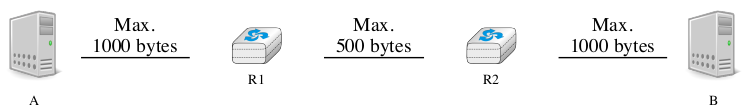
\includegraphics[width=12cm]{heterogeneous.png}
    \caption{Example of heterogeneous datalink layer}
\end{figure}

\subsubsection{Vitual circuit organisation}
TODO page 40

\subsubsection{The control plane}
There is two main technique that can be used to maintain the forwarding table in
a network : Distance vector routing and link state routing.

\subsubsection{Distance vector routing}
Allow router discover the destinations reachable inside the network as wall as
the shortest path to reach each of these destinations.
(\textit{each link as a associated cost})


\paragraph{Routing table contains} :
\begin{itemize}
    \item $R[d].link$ : outgoing link use to forward paquet to d
    \item $R[d].cost$ : cost of shortest path to d
    \item $R[d].time$ : time to last timestamp
\end{itemize}

\paragraph{Routing table update}
Router send regularly its \textbf{distance vector} over all interface.
If a router receiver a distance vector from link l, he only update
the corresponding entry  if either :
\begin{itemize}
    \item $V[d].cost+l.cost < R[d].cost$ : new route smaller thant route already know
    \item[OR]
    \item $R[d].link == l$ : Update of the same route
\end{itemize}

TODO page 46 (failure in distance vector routing)

\subsubsection{Link state routing}
Exchange messages to allow each router to learn the entier network topology, and so
each router is then able to compute its routing table by using a shortest path computation
\footnote{By Dijkstra}

\textbf{Weight} (\textit{Usually symmetric, but it's not a assumption}) of a link can be :
\begin{enumerate}
    \item Unit weight. (\textit{shortest path = lowest intermediate routers})
    \item Proportionnal to the propagation delay
    \item Opposite proportionnal of the bandwith ($\frac{C}{bandwith}$ where C is
    higher than the highest bandwith in the network)
\end{enumerate}

\paragraph{Routing table update}
TODO page 48

\subsection{Application}
%Big-little indian


\subsection{The transport layer}

La couche de transport doit gérer les problèmes de la couche network :
\begin{itemize}
    \item corrupt data
    \item loose data
    \item not deliver data in-order
    \item upper bound on maximun length of the data
    \item duplicate data
\end{itemize}

\subsubsection{Connectionless}
On envoi les données et le service assure qu'elle arrive.
Utilisé pour le transport de petit SDU.

\begin{description}
    \item[Reliable] : Garantit l'arrivée à coup sur des données. (\textit{difficile à mettre en pratique})
    \item[Unreliable] : Imperfection :
        \begin{itemize}
            \item Garantit seulement une majorité qui arrive (\textit{Souvent ce qui est écarté est du à l'overflow du buffer})
            \item Peut duppliquer les packets sur le réseau
            \item Peut délivrer un SDU différrents
            \item A une taille limité des données
        \end{itemize}
\end{description}
% Characteristic page 56

\paragraph{Note:} Pour passer du network layer au transport layer, il faut ajouter la
gestion des erreurs et une technique de multiplexing (\textit{via port}).


\subsubsection{Connection-oriented}
Ici il y a trois phases : établir la connection, transferer les SDUs (\textit{la connection est
bidirectionnel}) et fermer la connection.

\begin{description}
    \item[Reliability] : Elle n'est garantie que lorsque la connection est terminé avec un
        ``gracefully``, sinon des pertes peuvent être observé
\end{description}

\paragraph{Connection}

\paragraph{Refus:} Soit de la part du destinataire, soit du provider.

\paragraph{Three-way handshake} est utilisé contre l'approche naive de la connexion ``aller-retour''. Celle ci est définie par l'envoi d'un \textbf{CR}, répondu par \textbf{CA} qui répond \textbf{CA}.

Pour permettre le Three-way handshake, on utilise un transport clock.


\paragraph{Data transfert}

\paragraph{Mode}
\textsc{message-mode} : On envoie et reçois les messages tels quels.\\
\textsc{stream-mode} : On envoit içi des flux de bytes, et on a besoin de spécifié un délimiter
spécifique pour déliumiter les SDU dans le bytestream.

$\rightarrow$  Le \textbf{Stream-mode}  est utilisé  pour les  reliable
transport portocols,  et le  numéro de séquence  placé dans  la frame
correspond à la position du premier byte du payload dans le bytestream.

\paragraph{Note} : Plusieurs différence par rapport au datalink layer pour assurer que les
données soient délivré.

\begin{enumerate}
    \item Dans  le datalink  layer quand  deux host  sont
connecté le délai de transmission est fixe. Ici le delai varie car les
paquets envoyés  ne prennent pas  forcément le  même path et  il peut
être mis en attente dans le buffer d'un router.
    \item Les paquets n'arrivent pas tjrs en séquence contrairement au datalink layer
    \item Le network peut duppliquer les paquets dans le transport layer
\end{enumerate}

\paragraph{Solution} :
\begin{enumerate}
    \item Pour détecter les erreurs de transmission, comme dans le datalink layer, on utilise un
    CRC ou checksum sur \textbf{chaque} segment.
    \item Pour rendre le protocole reliable, on utilise un numéro de séquence et des numéro
    d'ackowledgement. (32 ou 64bits nécessaire plutot que 8 dans les datalinks layer protocol)
\end{enumerate}

\paragraph{Go-back-n and selective repeat}
Dans le transport layer on va préférer le sélective repeat puisque cette couche
ne garantit pas l'arrivée en séquence, contrairement au datalink layer.

De plus, dans le transport layer, plusieurs application concurrente peuvent communiquer
du coup l'espace mémoire offer à chaque application peut varier ce qui peut rendre la
taille du buffer variable.
Le sender à un swin (\textit{taille de son buffer}), et rwin (\textit{taille du buffer du receiver}). Il considère le minimun des deux comme la window size.


\textbf{Pour éviter un deadlock}, on utilise un persistent timer lorsque le sender reçoit une
window size du receiver égale à 0. Quand le timer expire on force le renvoi du dernier segment.

\paragraph{Connection release}
Soit de manière \textbf{abrute}, soit de manière \textbf{gracefully} càd en fermant
les deux sens de la connections avec un DR suivit d'un ACK.


\subsubsection{Request-response service}

Page 61

\subsection{Naming and addressing}

\subsubsection{Benefit}

\subsection{Sharing ressources}

\textsc{bandwith} est la ressource la plus importante dans un réseau.\\
\textsc{buffer of network node} est une autre ressource importante.\\
\textsc{Processing capacity} to analyse packet and see on forwarding table.

\subsubsection{Organisation to sharing bandwith}

\paragraph{A full mesh}
Le plus efficace, mais nécessite $\frac{n \times (n-1)}{2}$ lien, et chaque
host doit manager $n-1$ interface ce qui peut vite devenir impossible.

\paragraph{Bus organisation}
Le danger est que si le cable du bus est coupé en deux, le réseau est scindé
ce qui peut être dur à maintenir.

\paragraph{Star organisation}
Le noeud du centre de l'étoile est vital pour le réseau, mais il permet aussi
de centraliser le control en un seul point (\textit{C'est un excellent point de
control et un bon point d'observation}).

Beaucoup plus facile à maintenir que le bus.


\paragraph{Ring organisation}
Un lien coupe l'entièrete du réseau, c'est pouquoi on utilise souvent un dual-ring.

\paragraph{Tree organisation}
Cela permet de connecté un large nombre de client avec un très petit coût.


\subsubsection{Sharing bandwith}

Le partage de bandwith dans les réseaux se veut être \textbf{max-min fairness}.

\paragraph{ }Plusieurs algorithme sont expliqué dans la section Medium Access Control.

\subsubsection{Network congestion}

Congestion lorsque $\sum demand > capacity$.

\paragraph{Congestion collapse}
Cela arrive lorsque le réseau est un peu congestionné, et donc la transmission est ralenti.
Si un protocole tel que \textsc{selective repeat} est utilisé, alors le sender peut
croire que le packet est perdu et donc renvoyé le packet ce qui ne fait qu'augmenter
la congestion!


Pour régulere la congestion, une solution est de connaître la congestiona actuel afin que
les hosts ajuste leur bandwith disponible pour diminuer la congestion.

Tant que le buffer est peu ou pas du tout rempli, cela signifie que la demande est plus
petite que la capacité et que le buffer sert juste à \textit{lisser} les demandes dans le temps.


\paragraph{Discard mechanism}
On peut choisir d'écarter des paquets qd le buffer est full ou plutot quand il
augmente dangereusement afin de prévenir une congestion!
Toutefois, discard a packet est la solution finale.

\begin{enumerate}
    \item Discard celui qui arrive. C'est le plus utilisé mais il tend à rester congestionner et
        les applications temps réelles en souffre bcp
    \item Discard le premier de la file est plus judicieux qu'il n'y parait puisque ce paquet
        y est depuis lgtps et on a surement déja détecté la perte (de part la congestion) avant!
    \item Random early discard permet de supprimer les paquets de différents flow en proportion
        à leur bandwith.
\end{enumerate}

Attention, supprimer un paquet est pas la meilleur solution puisqu'on supprime un paquet
qui a consommé des ressources alors qu'on manque justement de ressource!

\paragraph{Forward Explicit Congestion Notification}
Pour les réseaux datagramme,
on utilise un bit pour marquer si le paquet est passé par un endroit congestionné,
et si c'est le cas le receiver envoi un paquet pour informer le sender du degré
de congestion (càd $\frac{nbr congestion}{nbr paquet}$)

\paragraph{Backward Explicit Congestion Notification}
Même technique pour les réseaux virtuels, sauf qu'on marque l'acknowledgement.

\paragraph{Control packet}
TODO

\paragraph{Scheduler mechanism}
Permet d'attribuer une FIFO par flow et un round robin choisit le prochain paquet


\subsubsection{Distributing the load across the network}

\paragraph{Virtual network}
Ici lorsque un host veut envoyer une information, il spécifie la destination et parfois la
bandwith nécessaire. On lui répond si il peut ou non se connecter.. Cette technique
est utilisé notament par les téléphones.

\paragraph{Datagram network}
La technique du virtual ne peut être appliqué car dans le datagram un host n'a pas
besoin d'autorisation pour envoyer des packets.

TODO page 82


\paragraph{Shared popular file}

\paragraph{Save on multi server}

\paragraph{Using popular bittorent service}


\subsubsection{Congestion control}

Pour supprimer la \textbf{congestion collapse}, les hosts doivent réguler leur taux
de transmission. (\textit{Note qu'il y a d'autre méchanisme pour réguler tel que celui
basé sur les crédits})

Goals of congestion control for a set of i hosts :
\begin{itemize}
    \item Doit supprimer la congestion càd $\forall_t \sum r_i(t) \leq R$
    \item Efficace càd $\forall_t \sum r_i(t) \approx R$
    \item Juste pour tous (max-min fairness est l'utopie)
\end{itemize}

Le control de congestion est un algorithme qui adapte le taux de congestion :
\begin{enumerate}
    \item Multiplicative decreasing si il y congestion : $rate = rate*\beta, \beta <1$
    \item Additive increasing sinon :  $rate =  rate + \alpha, \alpha>0$
\end{enumerate}

\paragraph{Congestion control in window-based transport protocol}
TODO

\subsection{The reference models}

\begin{description}
    \item[Application] : \textsc{SDU}
    \item[Transport] : connectionless/connection-oriented, \textbf{souvent unreliable}, \textsc{segment}
    \item[Network] : connect to network pas forcément directly, , \textsc{packet}
    \item[Datalink] : directly connect device, \textbf{reliable or unreliable}, \textsc{frame} with variable or fixed length
    \item[Physical] : directly connect device, \textbf{Unreliable}, \textsc{bit}
\end{description}


\section{Protocols}

\subsection{Application layer}
TODO

\subsection{DNS}
Structure DNS message page 113.

DNS permet d'obtenir l'adresse qui correpond à un certain nom, mais on peut
faire un reverser DNS pour obtenir le nom d'une adresse.

\subsection{Electronic mail}

\subsubsection{Email message}
\textsc{Header:} (\textit{From, Date, To, Subject,  cc, bcc}) and \textsc{Body}

Line to separate header and body is empty and contains only CR and LF.

\subsubsection{Header field to support Multipurpose Internet Mail Extension}
Header line :
\begin{itemize}
    \item MIME-version : version de MIME pour l'encodage du mail
    \item Content-type : Type de donnée du message
        \begin{enumerate}
            \item multipart/mixed : le fichier contietn des parties d'encodage
                indépendant (text, binaire séparé dans le body par une line vide)
            \item multipart/alternative : même message avec différentes représentation
        \end{enumerate}
    \item Content-transfert-encoding : Comment le message est encodé
\end{itemize}

\subsubsection{The Simple Mail Transfer Protocol}

\subsection{HTTP}
Utilise des liens hypertext pour lier un fichier à un autre.

\paragraph{Trois composant du world wide web}
\begin{enumerate}
    \item \textsc{uniform resource identifiers} : URI désigne une ressource sans aucune ambiguité
sur le world wide web. (page 126)
    \item \textsc{html}
    \item Le protocol \textsc{http} composé de request (\textit{method, header, MIME document}) et response(\textit{status line, header, MIME document}).
\end{enumerate}

Page 129 pour les header fields.


Une requête \textsc{http} doit être \textbf{self-content}. Cependant, il est possible que
le serveur veulent personnaliser les réponses au préférence du client. Trois solution :
\begin{enumerate}
    \item En forçant le client à s'identifier (user/password is deprecated)
    \item TODO
    \item En utilisant des cookies
\end{enumerate}

\subsection{Remote Procedure call}
C'est comme appelé une procédure dans un code, sauf que l'on est pas sur
un host seul mais dans le réseau.

\paragraph{Encoding data}
\textsc{xdr} (\textit{plus efficace}), \textsc{json} (\textit{plus lisible}),\ldots

\paragraph{Reaching the calle}
Un mécanisme simple est \textsc{json-rpc} qui peut être utilisé en connectionless ou
connection-oriented, composé d'une requête et d'une réponse. (page 136)

\subsection{Internet transport protocols}
TODO page 137

\subsection{The User Datagram Protocol (UDP)}

C'est un unreliable connectionless transport service, au dessus d'une unreliable
connectionless network service, qui utilise les ports
pour permettre de communiquer avec plusieurs application et qui a comme
caractéristique :
\begin{itemize}
    \item SDUs doit être < 65467bytes
    \item Garantit pas que le SDU est délivré
    \item Ne peut pas délivré un SDU corrompu
\end{itemize}

\paragraph{Header} = Source port (16), dest port (16), length (16) et checksum (16)

\paragraph{Port} : 0 - 1023 (\textit{privileged}), 1024 - 49 151 (\textit{registered}),
49 152 - 65 535 (\textit{ephemere})

TODO paragraph page 139

\subsection{The transmission control protocol (TCP)}

Bi-directionnal bytestream d'une connection-oriented transport service, au dessus d'une unreliable connectionless network service.

(Window-based transport protocol using go-back-n)

\paragraph{Header} = Source port (16), dest port (16), sequence number (32), ack number (32),
window size (16), checksum (16)

\subsubsection{TCP connection etablishment}
Three-way handshake utilisant sequence number, ack number et SYN flag.

\begin{figure}[!ht]
  \centering
  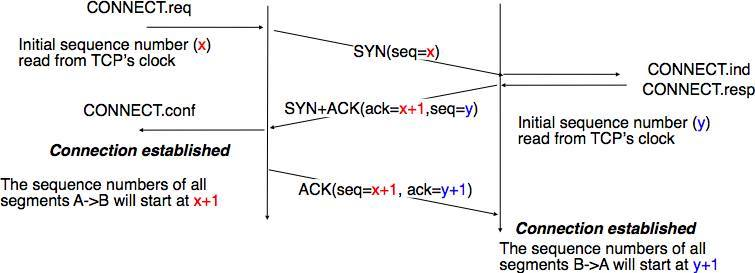
\includegraphics[width=10cm]{tcpconnect.jpg}
  \caption{Connection TCP}
  \label{fig:tcpconnect}
\end{figure}

Durant l'établissement de la connection, le client/serveur negocie plusieurs options :
\begin{enumerate}
  \item Le \textsc{mms} qui est la taille du plus grand payload acceptable (\textit{536 au minimun})
  \item La taille de la window
  \item L'utilisation de SACK
  \item Un ensemble d'option où client/server disent respectivemtn ce qu'il veut et ce
    qu'il supporte
\end{enumerate}

\paragraph{Encodage des options} est fait en \textsc{TLV}.

\subsubsection{TCP reliable data transfert}

\paragraph{Segment transmission strategie}

Deux solutions extrêmes :
\begin{enumerate}
    \item Première solution, envoyer quand on a besoin, mais cela peut impliquer d'envoyer
        un byte d'information avec 20 byte d'header\ldots pas très efficace
    \item L'autre extreme est d'envoyer qd on a rempli \textsc{mms} byte of data
\end{enumerate}

\paragraph{Nagle  algorithm}  :   on  envoi  le  paquet   si  il  rempli
un  \textsc{mms}  ou  si  l'on  vient  de  recevoir  un  acknwoledgement
(\textit{càd au moins à chaque round trip time}).

\subsubsection{TCP window}

La négociation du  window scaling factor ($0 \leq scaling  \leq 14$) se
fait  à la  connection, même  si certaines  implementations permettent
d'automatiquement ajuster la taille.

\subsubsection{TCP retransmission}
\textit{Go-back-n} a besoin d'un bon timer de retransmission (\textsc{rtt} est une
bonne estimation même si il change pdt la connection)

\textsc{rtt} = $\approx$ delai entre la transmission d'un segment et la reception de l'ack
\paragraph{Measure RTT }
Le problème est que l'on ne sait pas de quel segment l'ack est la réponse (càd qu'il pourrait
y avoir plusieurs segment identique envoyé)

Pour cela on utilise le \textbf{timestamp option} :
\begin{itemize}
    \item \textsc{ts} : Par exemple valeur de la clock
    \item \textsc{ts} echo : Dernier \textsc{ts}val reçu\\
\end{itemize}


Comme y'a plus d'ambiguité, on peut mettre à jour la valeur du time (\textit{souvent à 3sec
de base}).

\begin{itemize}
    \item \textsc{srtt} (\textit{smoothed rtt mcomputed}) = $ (\alpha \times srtt) + (1-\alpha) \times rtt)$, $rtt$ est le \textsc{rtt} measured
    \item \textsc{rto} (\textit{retransmission timedout}) = $min(60, max(1, \beta \times srtt))$, 1 et 60 sont les bornes minimal/maximal
\end{itemize}

\paragraph{Jacobson's algorithm} : en pratique ça marche pas bien, donc jacobson a une
autre idée, il redéfini \textsc{rto} = $srtt + 4*rttvar$ avec \textsc{rttvar} = $(1-\beta) \times rttvar + \beta \times |srtt - rtt|$.

$\beta = \frac{1}{4}, \alpha = \frac{1}{8}$

\subsubsection{Advanced retranmission strategie}

\paragraph{}
\textsc{tcp} utilise de base \textbf{go-back-n}, et lorsque le même timer
expire on recommande de doubler le timer (appellé \textit{exponential backoff}) jusqu'à
ce qu'il ait atteint 60sec où le host est considée inateignable.

\paragraph{delayed acknowledgement strategy}
Par ailleurs, il est aussi possible de perdre bcp de performance en envoyant des
ack quand il n'ont pas bcp d'interet. Typiquement, il est possible d'implémenter
un \textbf{delayed acknowledgement strategy} qui assure d'envoyer un ack a chaque fin
de timer (\textit{delai cour}) ou si il reçoit un segment hors séquence puisque du coup
l'ack a énormément d'importance

\paragraph{Out-sequence}
Il est très facile pour le receiver d'ajouter un buffer pour récupérer les
segments hors séquence sans avoir besoin d'en informer le sender.

\paragraph{Fast retransmit}
Actuellement, lorsqu'un segment est perdu il faut attendre que son timer expire
pour pouvoir le renvoyer. Une autre méthode consiste à détecter l'erreur lorsque
l'on reçoit 3 ack portant sur le même segment.

Il nécessite l'ajout d'une variable dubpacks dans le \textsc{tcb}.

\paragraph{Selective repeat}
Avec une option de TCP, on peut activer les \textbf{SACK} qui permettent d'indiquer
les segments qui ont été reçu hors séquence. On utilise ici souvent Fast retransmit avec.

\subsubsection{TCP connection release}
Abrut (\textsc{rst}) ou gracefully.
TODO page 156

\subsection{The stream control transmission protocol (SCTP) }
Alternative au TCP qui offre :
\begin{enumerate}
    \item Supporte efficacement the \textit{multihomed host} càd avec plusieurs interface réseau. En TCP, une IP par interface et si tu te connecte en WIFI puis que ça
        crash la connection ne sait pas être reprise par la 3G.
    \item La possibilité de pouvoir envoyer des messages par bytestream
    \item Partially-reliable
    \item Une seule vrai connection avec des streams \textit{logique} pour éviter de manager
        plusieurs connection
\end{enumerate}

\subsubsection{Segment}
C'est un header suivit d'un ensemble de chunk.

\paragraph{Header} = Source port number (16), dest port number (16), verification tag (32) and checksum (32).

\paragraph{Chunk} = Type (8), flags (8), length (16) et value (32) pour permettre d'insérer facilement un ensemble d'option. STCP, contrairement à TCP, n'est pas limité sur le nombre d'option. C'est bon exemple de format de protocol facilement etendable.

\subsubsection{Connection etablishment}
C'est un four-way handshake (pour contrer l'attaque ``Denial attack'')

TODO image

\subsubsection{Reliable data transfert}

\paragraph{Data chunck}
Les données sont envoyé via des \textbf{data chunck} qui utilise un TNS comme
numéro de séquence (augmenter de 1 a chaque data chunck). Lorsqu'un chunck est
scindé on utilise le bit \textsc{b} et \textsc{e} pour spécifier le premier et dernier
chunck.

\paragraph{Sack chunk}
Pour garantir l'arrivé, un TNS ack cumulatif est utilisé (Is on chunck level and not
byte level). Il donne aussi des informations sur les chunck hors séquence.
Plusieurs autre différence :
\begin{enumerate}
    \item Il peut fournir de l'information sur différent ``trou'' dans le buffer de réception
    \item Il peut donner un feedback sur chunck dupplicate (Annonce une mauvaise heuristic du sender)
\end{enumerate}

\subsubsection{Connection release}
Applique un three-way handshake pour cloturer la connection.
TODO error

\subsection{Congestion control}
Le control est effectué dans la transport layer.

\textsc{tcp} control la congestion en agissant sur la window size puisque une connection
ne peut pas envoyer des données plus vite que $\frac{window}{rtt}$

\paragraph{Congestion window}
\textsc{cwnd} est stocké dans le \textsc{TCB} de chaque connection, et la taille de la window
est $min(cwnd, rwin, swin)$.  \textit{Additive increase} : Chaque \textsc{rount trip time}, on incremente \textsc{cwnd} de MSS byte. \textit{Multiplicative decrease} : Quand une congestion
est detecté on divise \textsc{cwnd}.

\paragraph{Initial value cwnd}
est de MSS bytes afin de ne pas congestionner le réseau au démarrage.
(Cette valeur de départ a été augmenter à 15Kbyte)


Toutefois, cwnd va augmenter lentement avant d'arriver a une valeur qui utilise efficacement le
reseau. Pour éviter cela, on inclu un \textsc{slow-start algorithm} qui permet durant ce temps
de doubler \textsc{cwnd} chaque RTT.

\paragraph{Detect congestion} revient à detecter la perte de packet.
\begin{itemize}
    \item \textit{mild congestion} : Si on effecture un fast retransmit
    \item \textit{severe congestion} : Quand le timer de transmission expire
\end{itemize}

\begin{figure}
    %\includegraphics
    TODO image
   \caption{Congestion window with congestion}
\end{figure}

\subsubsection{Controlling congestion without losing data}
L'idée est de détecter avant la perte de paquet la futur congestion avec un
\textbf{Explicit Congestion Notification}. (Quant un paquet passe par un router
congestionné on met le bit à 1 et quand le receiver à cette information il la
transmet au sender pour adapter son débit)

\paragraph{}
\begin{enumerate}
    \item Pour déployer la solution, il faut un autre bit pour spécifier si le packet utilise
        ECN ou non. En effet, le cas échéant lorsque le router est congestionné ceux qui
        n'implémente pas ECN sont avantagé
    \item Si le protocol est reliable ont peut informer le sender via l'ack. Soit via
        un flag dans le header soit via une option. TCP``choisi le flag, STCP l'option.
    \item Dernièrement, le sender/receiver savent si il utilise ECN via une TCP option
        durant le three-way handshake de connection
\end{enumerate}

Si le receiver detect une congestion, les prochain paquets envoyé auront cette information.
(Pour éviter que l'information ne se perde si l'ack est perdu)

\paragraph{Router algorithm}
Deux types de router, soit avec une FIFO soit un ensemble de FIFO et round robin scheduler.

Au lieu de prendre une mesure instantanée du remplissage du buffer, on prend une moyenne
du remplissage.
De plus, chaque paquet à une probabilité d'être marqué comme congestionné qui augmente
quand la moyenne augmente.

\paragraph{}
Quand il y a plusieurs queue ont fait cette probabilité de manière indépendante pour
garantir la justesse.

\subsubsection{Modeling TCP congestion control}
TODO

\subsection{Network layer}
Trois type de datalink layer :
\begin{enumerate}
    \item Utilise directement le lien physique du physical layer
    \item Utilise un Local Area Network
    \item Utilise un Non-Broadcast Multi-Access (utilisé pour simuler une LAN supportant
        juste l'unicast)
\end{enumerate}

\paragraph{LAN} Dans une LAN Chaque host est identifié par un datalink layer adresse
(\textbf{MAC adresse}).
LAN supporte broadcast and multicast datalink layer adresses. Une frame envoyé a l'adresse
broadcast/multicast de la LAN est envoyé à tout les participants/participants correspondant
au groupe.

\subsubsection{IP version 6}
IPv4 ne pourra bientot plus supporter toute les adresses, d'ou le besoin
de passer à une autre solution.

\paragraph{IPv6 adressing architecture}
Support unicast, multicast and anycast.

\paragraph{Unicast}
TODO image 171

Une allocation hierarchique des allocations d'adresse permet de minimiser
le nombre de route connu par les router. Celui ci connait donc pour
certains block d'adresse!

$2^{128}$ groupé dans $2^{64}$ subnet!


Deux type d'allocation d'adresse :
\begin{enumerate}
    \item \textit{provider independent} (PI)
    \item \textit{provider aggregatable} (PA)
\end{enumerate}
TODO understand

\paragraph{Size IPv6 adress}
/32 = Internet Service Provider, /48 = single compagny, /56 = small user site,
/64 = single user, /128 = rare (Pas plus d'un host attaché au prefix)

\paragraph{Utilisation IPv6 prefix}
\textit{Longest prefix match} assure que la route qui match le plus avec
l'adresse est celle employé.

Note : ::/0 match avec tout le monde et est donc la \textit{default route}.

\paragraph{Link local unicast}
L'addresse commence par fe80::/64 et est suivi des 64 bits d'interfaces.
Utilisé quand deux host sur le même lien (or LAN) veulent échanger des
packet.. Note que le router ne peut pas forwarder un packet avec un
link local unicast.
(Utilisé qd on ne peut pas avoir une IPv6 régulière, càd en LAN isolé)


\paragraph{Multicast}
Envoyé efficacement un packet à toute les personnes d'une même groupe, dans une LAN.
TODO

\paragraph{IPv6 packet format}

\paragraph{No checksum}
Il n'y a pas de checksum dans le header de packet IPv6 car il y a déja le checksum
sur les frame au niveau datalink layer! En pratique, l'ajout d'un tel checksum prévient
les erreur de corruption de mémoire au sein d'un routeur (\textit{ridicule}) pour un coùt de
calcule élevé.

\paragraph{Next header}
Indique le prochain header, tel que un transport layer header (UDP, TCP, SCTP) ou une
IPv6 option (page 177). Note qu'une option a aussi le champ \textit{next header}.

\paragraph{Fragment option}
En IPv6 la fragmentation est fait par le sender et non par le router. (Celui-ci discard
le paquet et envoi un message d'erreur au sender si le packet est trop grand).

Un paquet fragmenté contient un numéro d'offset de la fragmentation, le next header (car une option), un champ réservé mis à 0, un flag pour dire si c'est le dernier fragment et un
champ pour \textit{identifier} le packet original.

\subparagraph{Note:} On peut envoyer les packets du premier au dernier ou dans l'ordre inverse.
La deuxieme solution permet au receiver de connaître la taille du paquet (et donc du buffer
nécessaire).

\subsubsection{ICMP version 6}
\textit{Internet Control Message Protocol} version 6 est utilisé dans un paquet IPv6
(next header = 58). Deux type de messages :

\begin{itemize}
    \item Messages d'erreurs
        \begin{enumerate}
            \item Destination unreachable (0: no route, 1: firewall refuse, 2: sender use link-local adresse to reach global unicast adresss, 3: adress unreachable, 4: port unreachable)
            \item Packet too big
            \item Time exceeded
            \item Parameter problem
        \end{enumerate}
    \item Messages d'information
\end{itemize}
TODO page 184

\subsection{The IPv6 subnet}
TODO

\subsubsection{Interactions between IPv6 and datalink layer}

Dans une LAN sans internet, les hosts prennent une adresse IP grace au link-local adresse.
Si la LAN est connecté à internet, on utilise \textit{Neighbor Discovery Protocol} (partie de ICMPv6) pour connaître l'adresse des autres

\paragraph{Neighbor Discovery Protocol}

\begin{enumerate}
    \item Envoi un multicast ICMPv6 Neighbor Solicitation avec son adresse IPv6
    \item Le receiver répond avec un ICMPv6 Neighbor Advertisement avec son adresse IPv6 et MAC
    \item En recevant le ICMPv6 NA, il stock le lien IPv6-MAC dans sa NDP table
\end{enumerate}
ICMPv6 NS peut aussi être utilisé pour voir si un host est atteignable. De plus, le ICMPv6 NA est
stocké temporairement dans la cache et quand il expire il faut revalider l'adresse.

\subparagraph{ }
\textit{Duplicate Address Detection algorithm} permet de ne pas avoir deux adresses identiques.
Pour cela il envoit un ICMPv7 NS à sonn adresse, et si il ne reçoit pas de réponse elle est
donc unique.

\paragraph{Automatically configure IPv6 adress}
\paragraph{Stateless Address Autoconfiguration} mechanism obtient sa link-local adresse
en prenant 64 bits concaténé avec fe80::/64 et en verifiant avec un NS son unicité.

\paragraph{ }
Obtenir  une   vrai  adresse  est   effectué  en  envoyant   un  Router
Advertissement  message  à  ff02::1  qui est  accessible  à  tout  les
local-link adresse.

\subparagraph{Option}
TODO page 189

\paragraph{Dynamic Host Configuration Protocol} (DHCP)
TODO

\paragraph{Multi router on subnet}
TODO



TODO image 189

\subsection{Routing in IP networks}
Deux classe de protocol entre les différents domaines pour echanger
efficacement de l'information.

Une grande différence entre intra et inter domaine est la \textit{routing policies}
utilisé par chaque domaine.

Dans un domaine toute les routers sont égaux et la meilleur route est choisi sur
différents critére : temps, nombre d'intermédiare et taille de bandwith.

\paragraph{Routing  policies}  =  import filter  (spécifie  les  routes
acceptables), export  filter (spécifies  les routes dangereuses)  et un
algorithme qui choisi.


\subsection{Intradomain routing}
Echange des informations sur les destinations atteignables \textbf{dans} le domain.
\textit{RIP} est protocol de distance vector et \textit{OSPF} utilise link-state routing.

\subsubsection{RIP}
Les routers echanges periodiquement des RIP messages (inside UDP segment).
Pour accélerer le processus (qd un router boot), il peut envoyer une RIP request à ff02::9
pour demander tout de suite les tables de routings (reçu via un RIP response).

\paragraph{RIP response} contiennent les distance vectors des tabels de routing.

\subsubsection{OSPF}

\paragraph{Area}
Avec le link-state routing, pour des grands réseaux c'est très couteux de stocker
l'ensemble du réseau en mémoire. C'est pourquoi on décompose le réseau en un
ensemble d'\textsc{area} où les routers connaissent la topologie de sa propre
région et comment rejoindre la \textit{backbone area}

\paragraph{Backbone area}
C'est l'area qui regroupe tout les \textit{border router} et ceux qui sont relié
à ces routers sans être dans une area.

L'inter-area routing est fait via un distance vector protocol.

TODO image page 195

\paragraph{LAN}
TODO point to point (R8-RC ? )

\paragraph{Shortest path}
TODO page 196

\subsection{Interdomain routing}
Echange de l'informations entre les domaines. Cette information est une information
agrégé des routers et on considère ici les domaines comme des boîtes noires.

\subsubsection{Connection}

\paragraph{Private peering link} permet de lier deux domaines. Pour des questions
de performances plusieurs lien physique sont établi entre les domaines.

\paragraph{Internet eXchange Point} Une solution moins couteuse est de les connecter
via un IXP. TODO page 198

\subsubsection{Connection cost} Le coût d'une route est très importante en interdomain
alors qu'en intra on préfére la performance.

Il existe deux types de relation entre domaine \textit{customer->provider} et \textit{
shared cost}.
TODO image page 198

\paragraph{customer->provider}
Le customer paye pour que son domaine soit distribué dans Internet

\paragraph{Shared cost}
Cela arrive quand on a des domaines de taille similaire

\paragraph{Sibling}
Ils échangenet les routes dans les deux directions (souvent c'est des routers
de la même compagnie).

\subsubsection{Interdomain routing policie}
TODO

\subsubsection{The Border Gateway Protocol (BGP)}
Dans BGP chaque domain est identifié par un unique \textit{Autonomous System} number (AS).

BGP n'envois pas sa routing table entière mais le fait de manière incrémentale, càd en
envoyant uniquement les routes qui ont changé.

De plus BGP utilise TCP pour garantir le bon délivrement des BGP messages.

\paragraph{BGP session}

\paragraph{Etablisment} doit être fait manuellement pour des raisons de sécurité.

\paragraph{Messages}

\begin{enumerate}
    \item \textit{OPEN} : Quand la connection est établie, ça initialise la session et
        négocie d'option
    \item \textit{NOTIFICATION} : Pour cloturer la session
    \item \textit{UPDATE} : Averti du changement d'une route. C'est le message le plus important et pour que le protocol soit efficace, le message doit minimiser le nombre de bit envoyé.
    \item \textit{KEEP ALIVE} : Averti que rien n'a changé (pour être sur que le router
        est toujours en vie)
\end{enumerate}

\paragraph{BGP update} = \{IP prefixe retié\}, \{IP préfixe ajouté\}, \{AS-Path\}

\subparagraph{ } Une route qui est envoyé doit d'abord passer l'\textit{export filter},
de même qu'une route reçue doit passer l'\textit{import filter}.
TODO

\paragraph{The BGP decision process}
En plus des import/export filter, il y a un algorithme qui choisit la meilleur route.
Ce choix est fait sur base des BGP attribut attaché à chaque route.

\paragraph{Local-pref}
Le premier attribut de cet algorithme est la local-preference, celui ci est attribué
selon l'import filter. (Highest value est préféré)

\subparagraph{Cheap link} On peut implémenté la préférence d'un lien peut couteux
plutôt qu'un autre via le local-pref en définissant les valeurs dans l'import filter.


\paragraph{Local-pref with customer->provider and shared cost}
\begin{enumerate}
    \item High local-pref pour les routes apprisent par le customer (\textit{provider->customer})
    \item Medium local-pref pour les shared-cose
    \item Low local-pref pour les routes apprisent par le provider (\textit{customer->provider})
\end{enumerate}


\paragraph{BGP convergence}
Certaines routing policies peuvent interférer entre elles et aboutir (en théorie),
à des ping-pong infini.

\paragraph{ } La convergence des BGP n'esy pas toujours garanti et verifier la
convergence global est un problème NP-complet.

\paragraph{Guideline to guarantee BGP convergence}
\begin{enumerate}
    \item Le graph est \textit{customer->provider} est acyclique
    \item AS préfére une route reçue d'un customer plutôt qu'une shared-cost
\end{enumerate}

\subsubsection{Structure global internet}
TODO page 209

\subsection{Datalink layer technologie}

\subsubsection{The point to point protocol}
Protocol dévellopé après me \textit{Serial Line IP} (SLIP) qui a beaucoup de limitation.

PPP est enfaite en famille de trois protocol :
\begin{enumerate}
    \item The PPP define framing technique to transport network layer packet
    \item The \textit{Link Control Protocol} est utilisé pour negociate option and authentification by username/password
    \item The \textit{Network Control Protocol} est spécifique à chaque network layer protocol
\end{enumerate}

PPP frame utilise le bit/caractère stuffing, supporte variable length (même si LCP négocie la MAX size).

\subsubsection{Ethernet}
TODO changement + slot time

\paragraph{Hubs}
Les hosts peuvent être directement relié à un Ethernet hubs.
\subparagraph{Complexe network hub} La topologie doit être un tree et le délai entre
deux host ne peut pas être plus long que 51.2ms (slot time).

\paragraph{Frame format}
TODO image page 213

\paragraph{Ethernet service}
Ethernet network offre un unreliable connectionless service qui supporte unicast, multicast et
broadcast.

En pratique il délivre les frames au destinataire avec une \textbf{TRES} grande probabilité,
et les frames arrivent en séquence.

\paragraph{Fast ethernet}
TODO page 215

\paragraph{Ethernet switches}
Augmenter la bande passante comme \textit{fast ethernet} n'est pas la seule
manière d'améliorer les performances d'ethernet LAN, on peut aussi rendre
les hubs intelligents en devenant des switchs.

Ceux-ci maintiennent une table de forwading pour les MAC adresses.

TODO image page 217


\paragraph{MAc adress}
Quand deux host sont sur le même hub/segment ethernet, ils peuvent échanger de
l'information sans configuration ce qui implique que un switche doit pouvoir
construire sa table de MAC adresse \textit{automatiquement}.

$\rightarrow$ Pour chaque frame reçue, la MAC adress est extraite de la frame et mise dans la table.

\paragraph{ }
The \textit{MAC adress learning} algorithm fonctionne bien sur un tree-shaped network,
sauf que cette topologie est dangereuse si l'un des switchs tombent en panne\ldots

Toutefois, si ce n'est pas un arbre ont peu rapidement tomber dans une boucle infinie
(si il n'y a pas de RTT ou Hop limit)!

\paragraph{Spanning tree protocol}
Désactive automatiquement des ports pour rester dans une tree-shaped, mais si l'un
des switchs crash, il y a un autre qui peut prendre le relais.

Le switch root est celui avec la plus petite MAC adress, ensuite le spanning tree est construit
pour que chaque switch ait le plus path vers le root.

Ils utilisent des BPDUs qui contiennent :
\begin{itemize}
    \item L'identifiant du root
    \item Le coût du path entre le root et celui qui envoit le BPDU
    \item L'identifiant de celui qui envoit le BPDU
    \item Le nombre de switch port par lequel il est passé
\end{itemize}


Durant la création du spanning tree toutes les data frames sont écarté
car on ne peut pas garantir l'absence de loop.


\paragraph{Virtual LAN}

TODO page 222

\subsubsection{802.11 Wireless networks}

TODO page 223

\biblio

\end{document}
